\title{Maya Soft Body Deformer Plugin Using Shape Matching \\ \large SFX - Tricks of the trade: Project Report}

\author{\begin{tabular}{ccc}
    Isabell Jansson & Ronja Grosz  & Jonathan Bosson \\
    \small isaja187@student.liu.se &\small rongr946@student.liu.se &\small jonbo665@student.liu.se \\
\end{tabular}}
\date{\today}

\documentclass[12pt, twocolumn]{article}
\usepackage{graphicx} % Figures
\usepackage{amsmath}

\begin{document}
\twocolumn[
\begin{@twocolumnfalse}
\maketitle

\begin{abstract}

\end{abstract}

\end{@twocolumnfalse}
]

\section{Introduction}

\section{Background}
    The shape matching approach followed was proposed by M\"uller et al.~\cite{shapematching}. 
    It is a shape matching technique for deformation of soft objects.
    
\section{Shape matching}

    \begin{figure}
    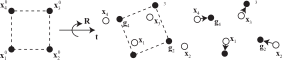
\includegraphics[width=\linewidth]{img/deformation2.png}
    \caption{The shape matching process where the original shape $\mathbf{x}^0_i$ is matched to the deformed shape $\mathbf{x}_i$ and pulled towards the goal shape $\mathbf{g}_i$. Image source:~\cite{shapematching}.}
    \label{fig:def}
    \end{figure}
   
    \begin{equation} \label{eq:min}
        \sum_i{w_i(\mathbf{R}(\mathbf{x}_i^0 - \mathbf{t}_0) + \mathbf{t} - \mathbf{x}_i)^2}
    \end{equation}

    \begin{equation} \label{eq:com1}
        \mathbf{t}_0 = \mathbf{x}^0_{cm} = \frac{\sum_i{m_i\mathbf{x}_i^0}}{\sum_i{m_i}}
    \end{equation}

    \begin{equation} \label{eq:com2}
        \mathbf{t} = \mathbf{x}_{cm} = \frac{\sum_i{m_i\mathbf{x}_i}}{\sum_i{m_i}}
    \end{equation}

    To find the optimal rotation matrix $\mathbf{R}$ the relative locations 
    $\mathbf{q}_i = \mathbf{x}^0_i - \mathbf{x}^0_{cm}$ and 
    $\mathbf{p}_i = \mathbf{x}_i - \mathbf{x}_{cm}$ are defined and the rotation matrix 
    $\mathbf{R}$ is approximated by finding the linear transformation $\mathbf{A}$, see equation~\ref{eq:A}.

    \begin{equation} \label{eq:A}
        \mathbf{A} = (\sum_i{m_i\mathbf{p}_i\mathbf{q}_i^{\mathbf{T}}})
        (\sum_i{m_i\mathbf{q}_i\mathbf{q}_i^{\mathbf{T}}})^{-1} 
        = \mathbf{A}_{pq}\mathbf{A}_{qq}
    \end{equation}

    \begin{equation}\label{eq:goal}
        \mathbf{g}_i = \mathbf{R}(\mathbf{x}^0_i - \mathbf{x}^0_{cm}) + \mathbf{x}_{cm}
    \end{equation}

    \begin{equation} \label{eq:vel}
        \mathbf{v}_i(t + h) = \mathbf{v}_i(t) + \alpha{\frac{\mathbf{g}_i(t) - \mathbf{x}_i(t)}{h}} + hf_{ext}(t)/m_i
    \end{equation}

    \begin{equation} \label{eq:pos}
        \mathbf{x}_i(t + h) = \mathbf{x}_i(t) + h\mathbf{v}_i(t + h) 
    \end{equation}

\section{Summary}\label{conclusions}

\bibliographystyle{ieeetr}
\pagebreak
\bibliography{./refs}

\end{document}
